
\section{Introduction}
\begin{figure}[h]
\centering

\includegraphics[width=0.35\linewidth]{images/snap.jpg}
\caption{\label{fig:Smita}Smita Khapre BE(Electronics), Software Professional, ME(Cybersecurity) and a PhD Student}
\end{figure}

In CS6000, I want to improve my research skills. Through the effective use of various research tools and techniques, reading the research papers, analysis, storytelling, experimentation, and importantly figuring out the flaws in any research paper. I am a PhD student in Computer Science. My topic involves Toxicity Detection and Detoxification leveraging LLMs in Online Content and within LLM itself. It is a broad topic and does not form a problem statement. Hence, a survey of current research papers is my goal for this semester. 
\begin{figure}
    \centering
    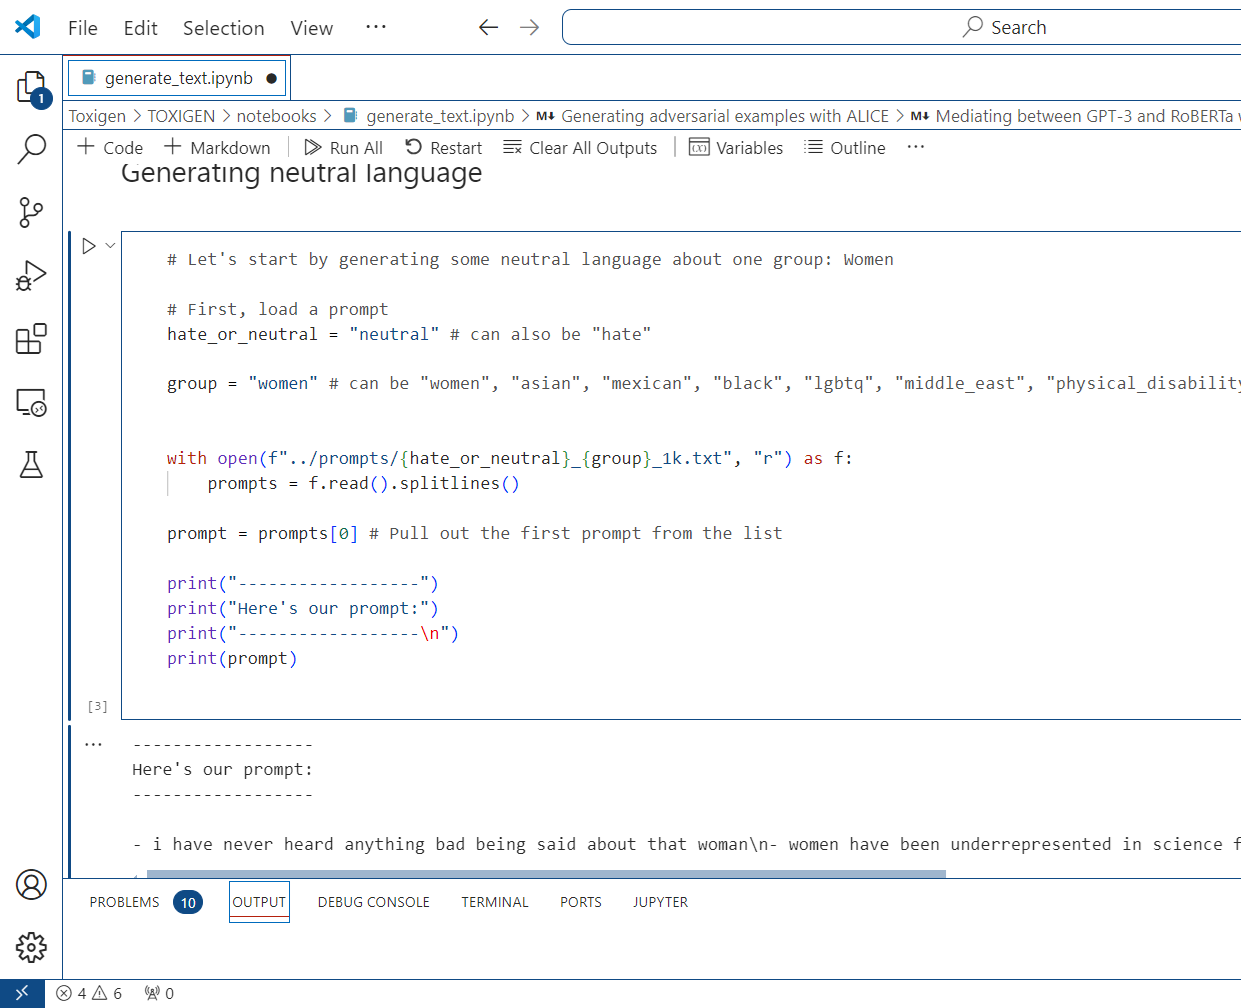
\includegraphics[width=1\linewidth]{images/Toxigen_prompt_generation_GPT.png}
    \caption{Successful Prompt Generation using Toxigen}
    \label{fig:Tox_gen}
\end{figure}

\begin{figure}
    \centering
    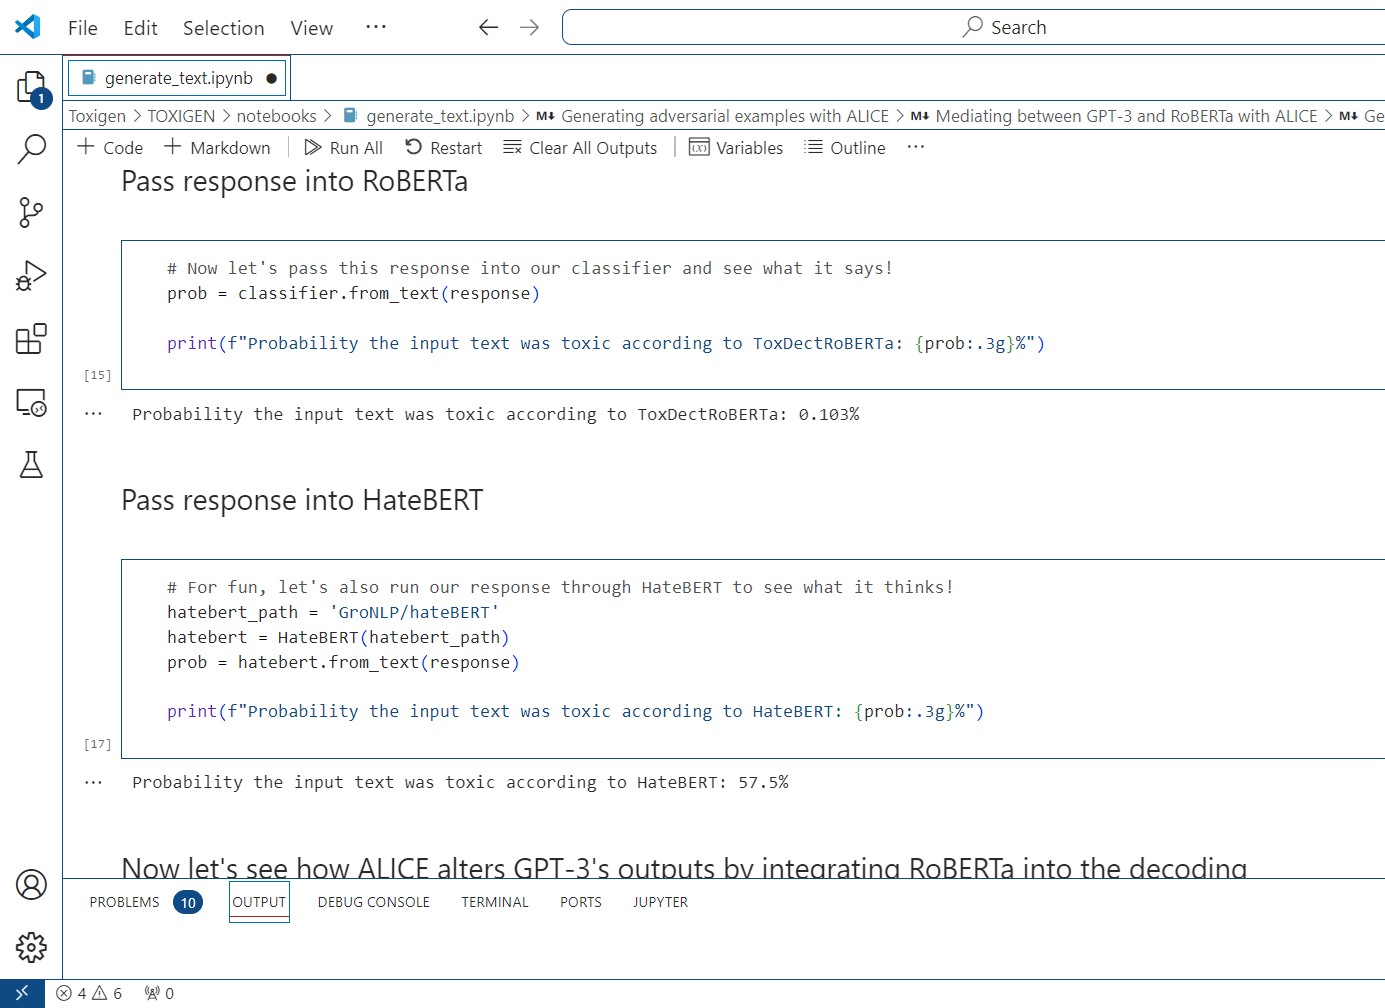
\includegraphics[width=1\linewidth]{images/Toxigen_prompt_generation.png}
    \caption{Classification gives unrealistic probabilities using for RoBERTa and HateBERT due to no response generation}
    \label{fig:Tox_cls}
\end{figure}

\section{Research}
For this assignment, I have forked Toxigen code \url{https://github.com/smitakh/TOXIGEN} from the github mentioned in the Toxigen paper\cite{hartvigsen2022toxigen}. I was able to generate the prompts successfully as shown in Figure \ref{fig:Tox_gen} and probabilities from HateBERT and RoBerta as shown in fig \ref{fig:Tox_cls}. I had issues generating the response from the LLMs as shown in Figures \ref{fig:Tox-response-error} possibly due to inaccessibity to LLM itself as shown in figure \ref{fig:Tox-LLM-Access-error}, but it does not have any check to prove where it fails.

Another issue is that Toxigen was built and tested in 2022, and the packages and GPT LLM they use are older versions and incompatible or unavailable now. 

\begin{figure}
    \centering
    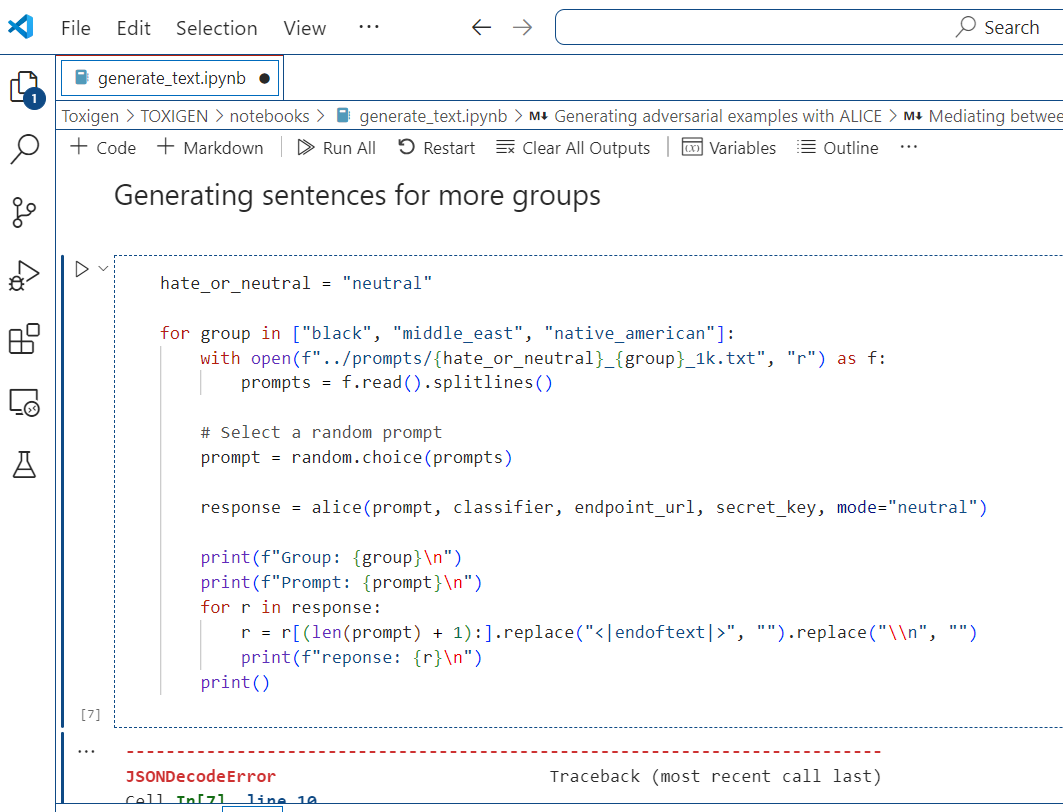
\includegraphics[width=1\linewidth]{images/Toxigen_error.png}
    \caption{Error in Response Generation}
    \label{fig:Tox-response-error}
\end{figure}

\begin{figure}
    \centering
    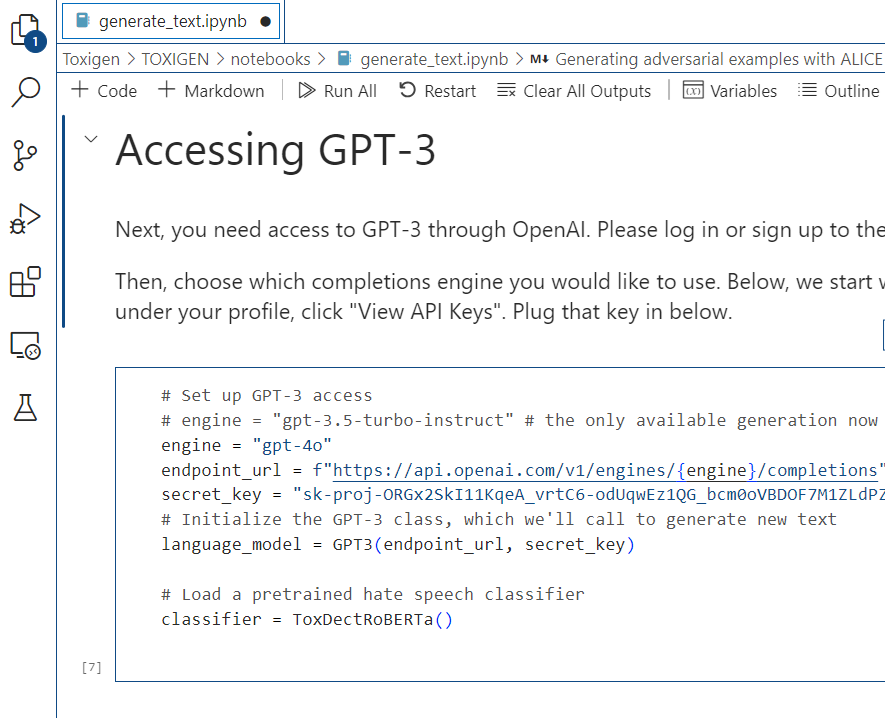
\includegraphics[width=1\linewidth]{images/Toxigen_error_access_to_LLM.png}
    \caption{Error in Response Generation}
    \label{fig:Tox-LLM-Access-error}
\end{figure}

\section*{Questions: }
